\documentclass[border=10pt]{standalone}
\usepackage{tikz}
\usepackage{wasysym}  % for \diameter symbol
\usetikzlibrary{arrows.meta, patterns, decorations.markings}

\begin{document}

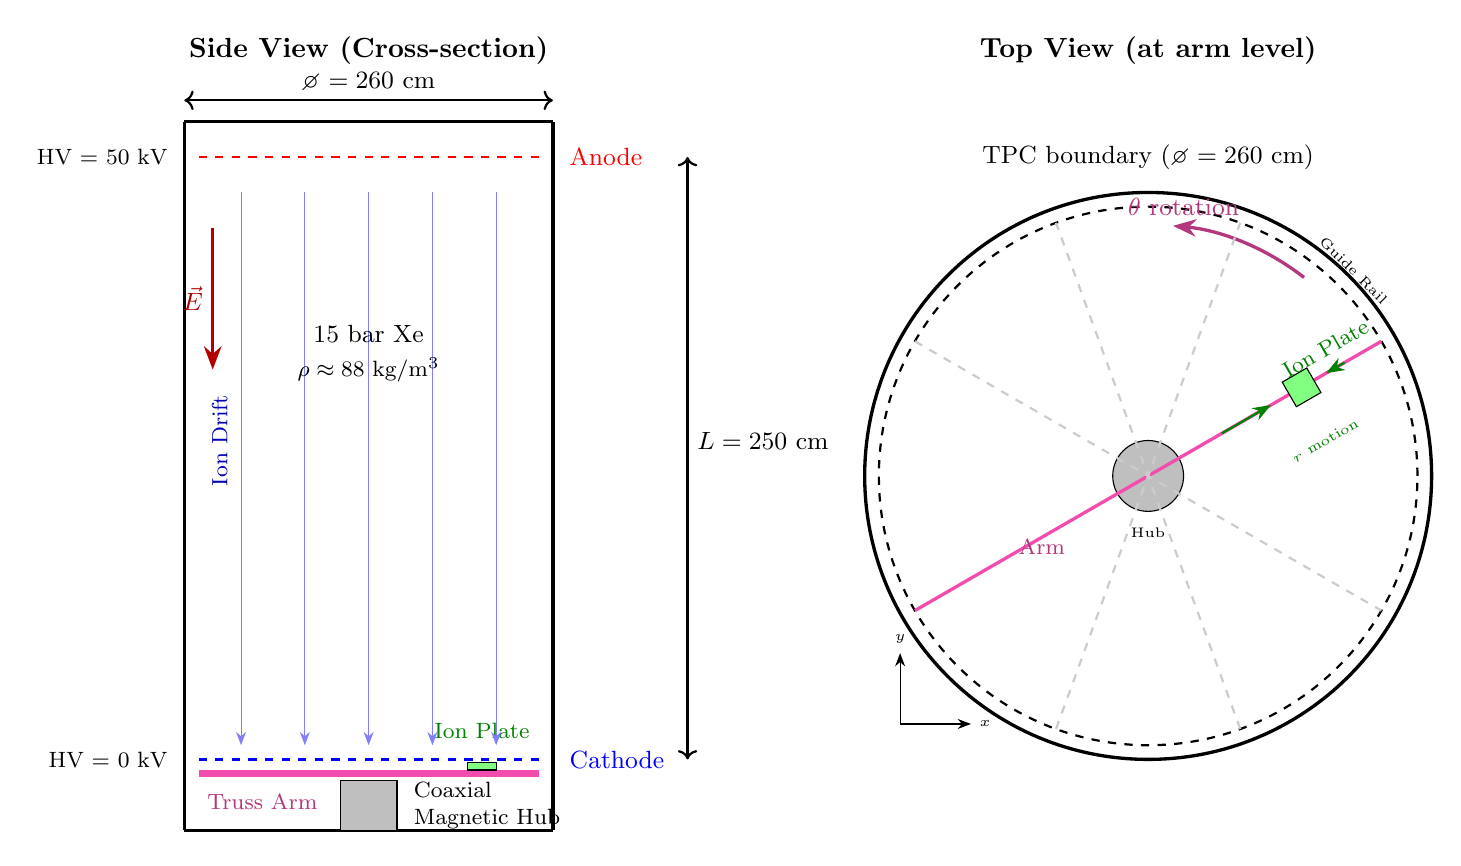
\begin{tikzpicture}[scale=0.9]

% === SIDE VIEW (Cross-section) ===
\begin{scope}[shift={(-6,0)}]
    \node[font=\bfseries] at (0,6) {Side View (Cross-section)};

    % TPC vessel walls (260 cm diameter x 250 cm length, scaled)
    \draw[very thick] (-2.6,-5) -- (-2.6,5);
    \draw[very thick] (2.6,-5) -- (2.6,5);
    \draw[very thick] (-2.6,5) -- (2.6,5);
    \draw[very thick] (-2.6,-5) -- (2.6,-5);

    % Anode (top) - dashed, HV = 50 kV
    \draw[thick, dashed, red] (-2.4,4.5) -- (2.4,4.5);
    \node[right, red, font=\small] at (2.7,4.5) {Anode};
    \node[left, font=\footnotesize] at (-2.7,4.5) {HV = 50 kV};

    % Cathode (above the truss) - dashed, HV = 0
    \draw[thick, dashed, blue] (-2.4,-4.0) -- (2.4,-4.0);
    \node[right, blue, font=\small] at (2.7,-4.0) {Cathode};
    \node[left, font=\footnotesize] at (-2.7,-4.0) {HV = 0 kV};

    % Coaxial magnetic hub (grey block at center bottom, shorter)
    \draw[fill=gray!50] (-0.4,-5) rectangle (0.4,-4.3);
    \node[right, font=\footnotesize, align=left] at (0.5,-4.65) {Coaxial\\Magnetic Hub};

    % Truss arm (pink thick line spanning full diameter, on top of hub)
    \draw[line width=2.5pt, magenta!70] (-2.4,-4.2) -- (2.4,-4.2);
    \node[below, font=\footnotesize, magenta!70!black] at (-1.5,-4.35) {Truss Arm};

    % Ion Plate (thin green rectangle, sitting on top of truss arm)
    \draw[fill=green!50] (1.4,-4.15) rectangle (1.8,-4.05);
    \node[above, font=\footnotesize, green!50!black] at (1.6,-3.85) {Ion Plate};

    % Dimension: TPC length
    \draw[<->, thick] (4.5,-4.0) -- (4.5,4.5);
    \node[right, font=\small] at (4.5,0.5) {$L = 250$ cm};

    % Dimension: TPC diameter (at top)
    \draw[<->, thick] (-2.6,5.3) -- (2.6,5.3);
    \node[above, font=\small] at (0,5.3) {$\diameter = 260$ cm};

    % Ion drift arrows (thinner lines, from anode toward cathode/plate)
    \foreach \x in {-1.8,-0.9,0,0.9,1.8} {
        \draw[-{Stealth}, thin, blue!50] (\x,4.0) -- (\x,-3.8);
    }
    \node[font=\footnotesize, blue!70!black] at (-2.1,0.5) {\rotatebox{90}{Ion Drift}};

    % Electric field
    \draw[-{Stealth}, very thick, red!70!black] (-2.2,3.5) -- (-2.2,1.5);
    \node[left, font=\small, red!70!black] at (-2.2,2.5) {$\vec{E}$};

    % Gas label
    \node[font=\small] at (0,2) {15 bar Xe};
    \node[font=\footnotesize] at (0,1.5) {$\rho \approx 88$ kg/m$^3$};
\end{scope}

% === TOP VIEW ===
\begin{scope}[shift={(5,0)}]
    \node[font=\bfseries] at (0,6) {Top View (at arm level)};

    % TPC circular boundary
    \draw[very thick] (0,0) circle (4);
    \node[font=\small] at (0,4.5) {TPC boundary ($\diameter = 260$ cm)};

    % Guide rail (dashed circle)
    \draw[thick, dashed] (0,0) circle (3.8);
    \node[font=\tiny, rotate=-45] at (2.9,2.9) {Guide Rail};

    % Central hub (grey)
    \draw[fill=gray!50] (0,0) circle (0.5);
    \node[font=\tiny] at (0,-0.8) {Hub};

    % Truss arm (pink thick line, current position)
    \draw[very thick, magenta!70, rotate=30] (-3.8,0) -- (3.8,0);

    % Ion plate (small green square, movable along arm)
    \draw[fill=green!50, rotate=30] (2.3,-0.2) rectangle (2.7,0.2);

    % Radial motion arrow (along arm)
    \draw[-{Stealth}, thick, green!50!black, rotate=30] (1.2,0) -- (2.0,0);
    \draw[-{Stealth}, thick, green!50!black, rotate=30] (3.2,0) -- (2.9,0);
    \node[font=\tiny, green!50!black, rotate=30] at (2.5,0.5) {$r$ motion};

    % Azimuthal rotation arrow
    \draw[-{Stealth}, very thick, magenta!70!black] (2.2,2.8) arc (52:85:3.5);
    \node[font=\small, magenta!70!black] at (0.5,3.8) {$\theta$ rotation};

    % Ghost positions of arm (showing rotation)
    \draw[thick, gray!40, dashed, rotate=70] (-3.8,0) -- (3.8,0);
    \draw[thick, gray!40, dashed, rotate=110] (-3.8,0) -- (3.8,0);
    \draw[thick, gray!40, dashed, rotate=-30] (-3.8,0) -- (3.8,0);


    % Coordinate system
    \draw[-{Stealth}] (-3.5,-3.5) -- (-2.5,-3.5);
    \draw[-{Stealth}] (-3.5,-3.5) -- (-3.5,-2.5);
    \node[font=\tiny] at (-2.3,-3.5) {$x$};
    \node[font=\tiny] at (-3.5,-2.3) {$y$};

    % Labels for key components
    \node[font=\footnotesize, magenta!70!black] at (-1.5,-1.0) {Arm};
    \node[font=\footnotesize, green!50!black, rotate=30] at (2.5,1.8) {Ion Plate};

\end{scope}

\end{tikzpicture}

\end{document}
